% Set the stage on AI systems
\label{sec:introduction:preface}

Within the last half-decade, we have seen an explosion of cloud-based services typically marketed under an \gls{ai} banner. 
Vendors are rapidly pushing out \gls{ai}-based solutions, technologies and products that encapsulate half a century worth of machine-learning research: a \citeyear{LoGiudice:2016wf} report by market research company Forrester captured such growth into four key areas \citep{LoGiudice:2016wf} as replicated in  \cref{fig:introduction:ai-products}. 
Moreover, developers eager to develop a next generation of software are shifting away from mobile-first to `\gls{ai}-first' apps, that will reason, sense, think, act, listen, speak and execute our whims right within the palms of our hands. 
A wave of \gls{ai}-first thinking embedded in companies' product lines is spearheaded through work achieved at Google, Microsoft and Facebook; for instance, Google's 2018 rebranding of \textit{Google Research} to \textit{Google AI} \citep{Howard:2018tz} or how \gls{ai} is leveraged \textit{at scale} within Facebook's infrastructure and platforms to serve its users with an \gls{ai}-first attitude \citep{Parekh:2017hx}.

\begin{figure}[thp]
\centering
\caption[Categorisation of AI-based products and services]{A Broad Range of AI-Based Products And Services Is Already Visible. (From \citep{LoGiudice:2016wf}.)}
\label{fig:introduction:ai-products}
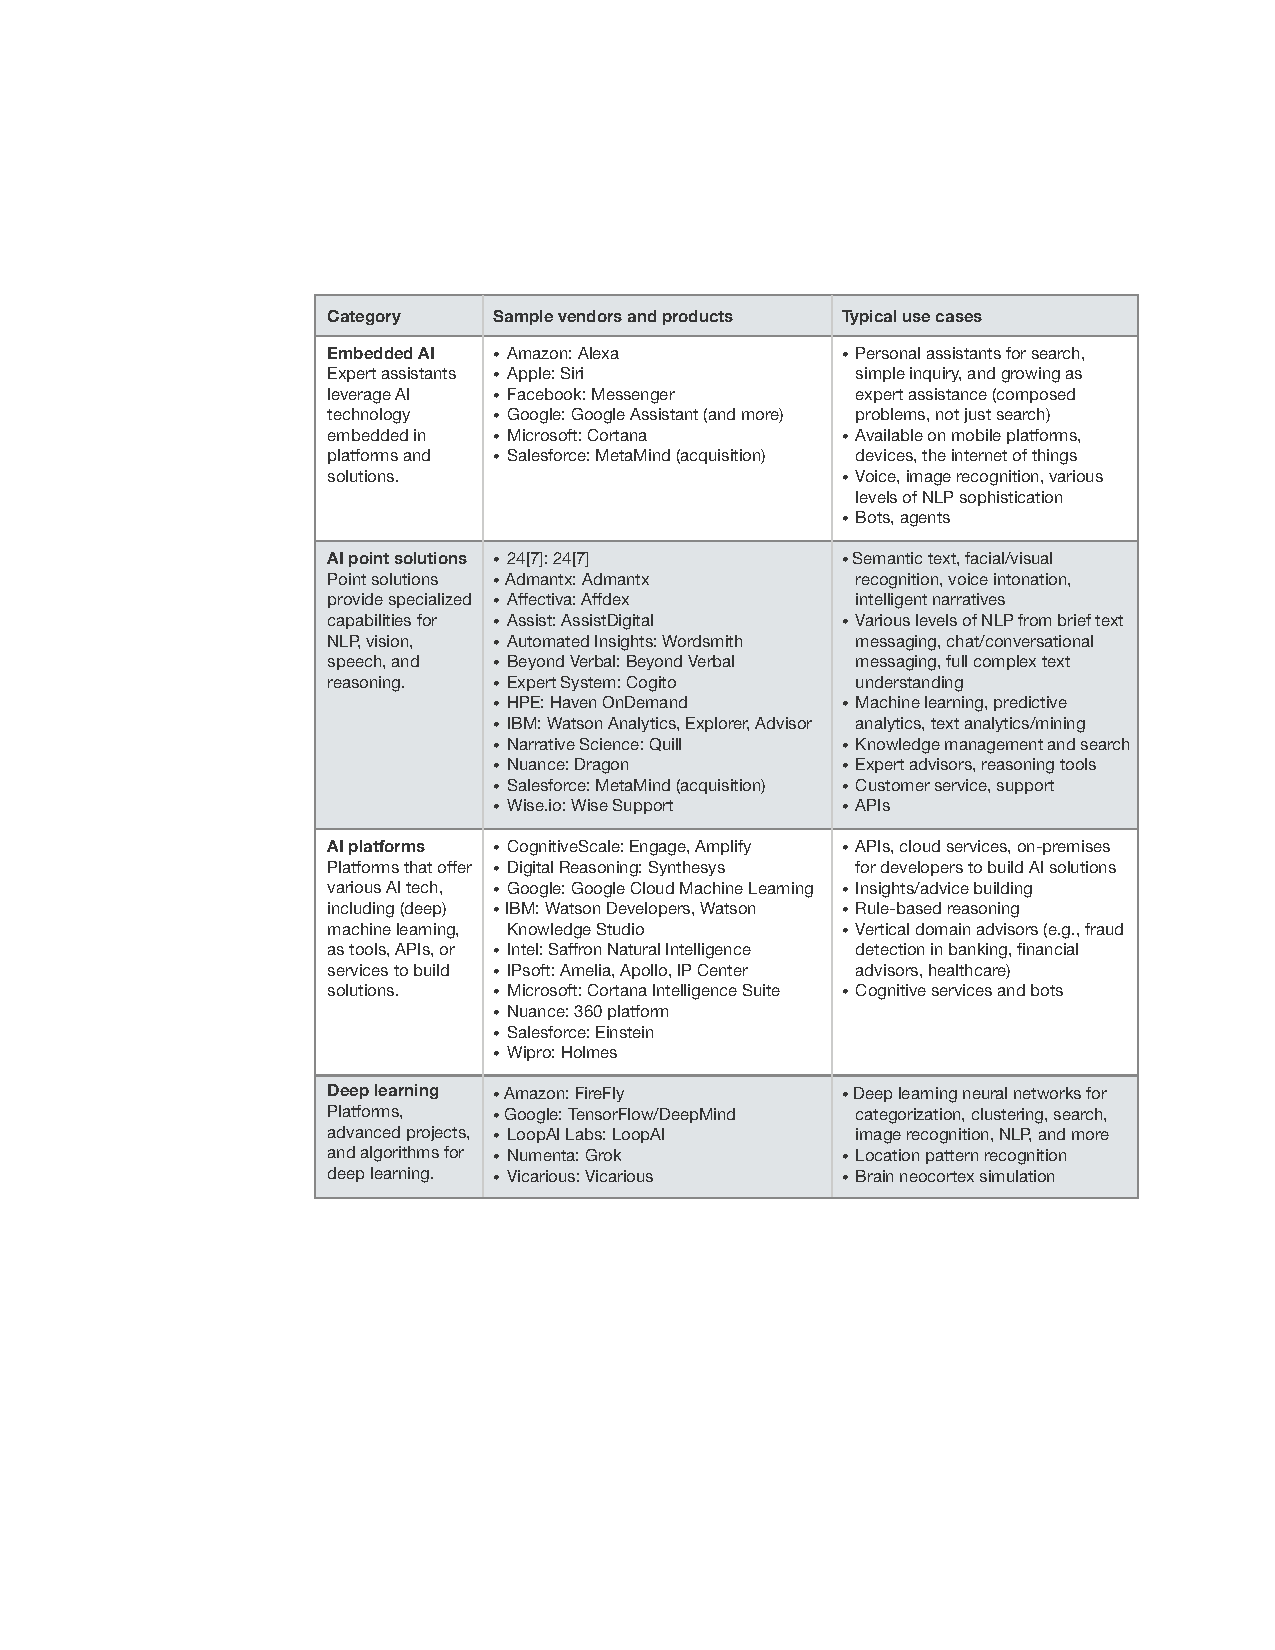
\includegraphics{ai-products}
\end{figure}

These services aim to lower the entry barrier to develop, test and deploy \gls{ai}-first software in both skill and time. 
Software engineers needn't require a formal training in machine-learning nor a strong understanding of mathematics: thus, \textit{skill required} is reduced. The training of such classifiers involves the laborious process of sourcing, curating and labelling large datasets: using such services does not, and thus \textit{time} is reduced. To this end, they needn't require much machine-learning expertise or experience at all; instead, the process is abstracted behind an \gls{api} call, only requiring knowledge on how to use a RESTful architecture \citep{Fielding:2000vh} to access the cloud service. 

To contrast this with more traditional means, a developer may choose to write up a deep-learning \gls{nn} (for example) and train it using their own dataset. While this is laborious in time and demands significant knowledge in machine learning, the developer has full control over the models she creates. Alternatively, she may choose to download a pre-trained model and \gls{ml} framework, such as Tensorflow \citep{Tensorflow:Whitepaper}; less demanding in time but still requiring the knowledge to wire-up models with frameworks.

With less time and skill required to build \gls{AI}-first apps using these cloud services,  these services have begun to gain traction within developer circles: \cref{fig:introduction:stackoverflow-trends} shows the increasing trend of posts since 2014 on Stack Overflow that categorise popular computer vision cloud APIs.\footnote{Query run on 12 October 2018 using StackExchange Data Explorer. Refer to \url{https://data.stackexchange.com/stackoverflow/query/910188} for full query.} A growing popularity into such `off-the-shelf' cloud services sparked varied nomenclature in academia: \textit{Cognitive Applications} and \textit{Machine Learning Services} \citep{Hwang:2017tr} or \textit{Machine Learning as a Service} \citep{Ribeiro:2015dz} are some coined phrases in which the intelligence is provided or created as a service via the cloud. Some of these services provide the infrastructure to rapidly begin training from custom datasets (Google's AutoML\footnoteurl{https://cloud.google.com/automl/}{7 December 2018} is one such example) while others provide pre-trained datasets `ready-for-use' in production without the need to train data. We refer to these latter services under the broader term `Cloud Intelligence Services' (\glspl{CIS}), and diagrammatically express their usage within \cref{fig:introduction:cloud-intelliegnce-service}.

\begin{figure}[t]
\centering
\caption[Increasing interest in the developer community of computer vision APIs]{Number of posts categorised on Stack Overflow under popular computer vision cloud intelligence services.}
\label{fig:introduction:stackoverflow-trends}
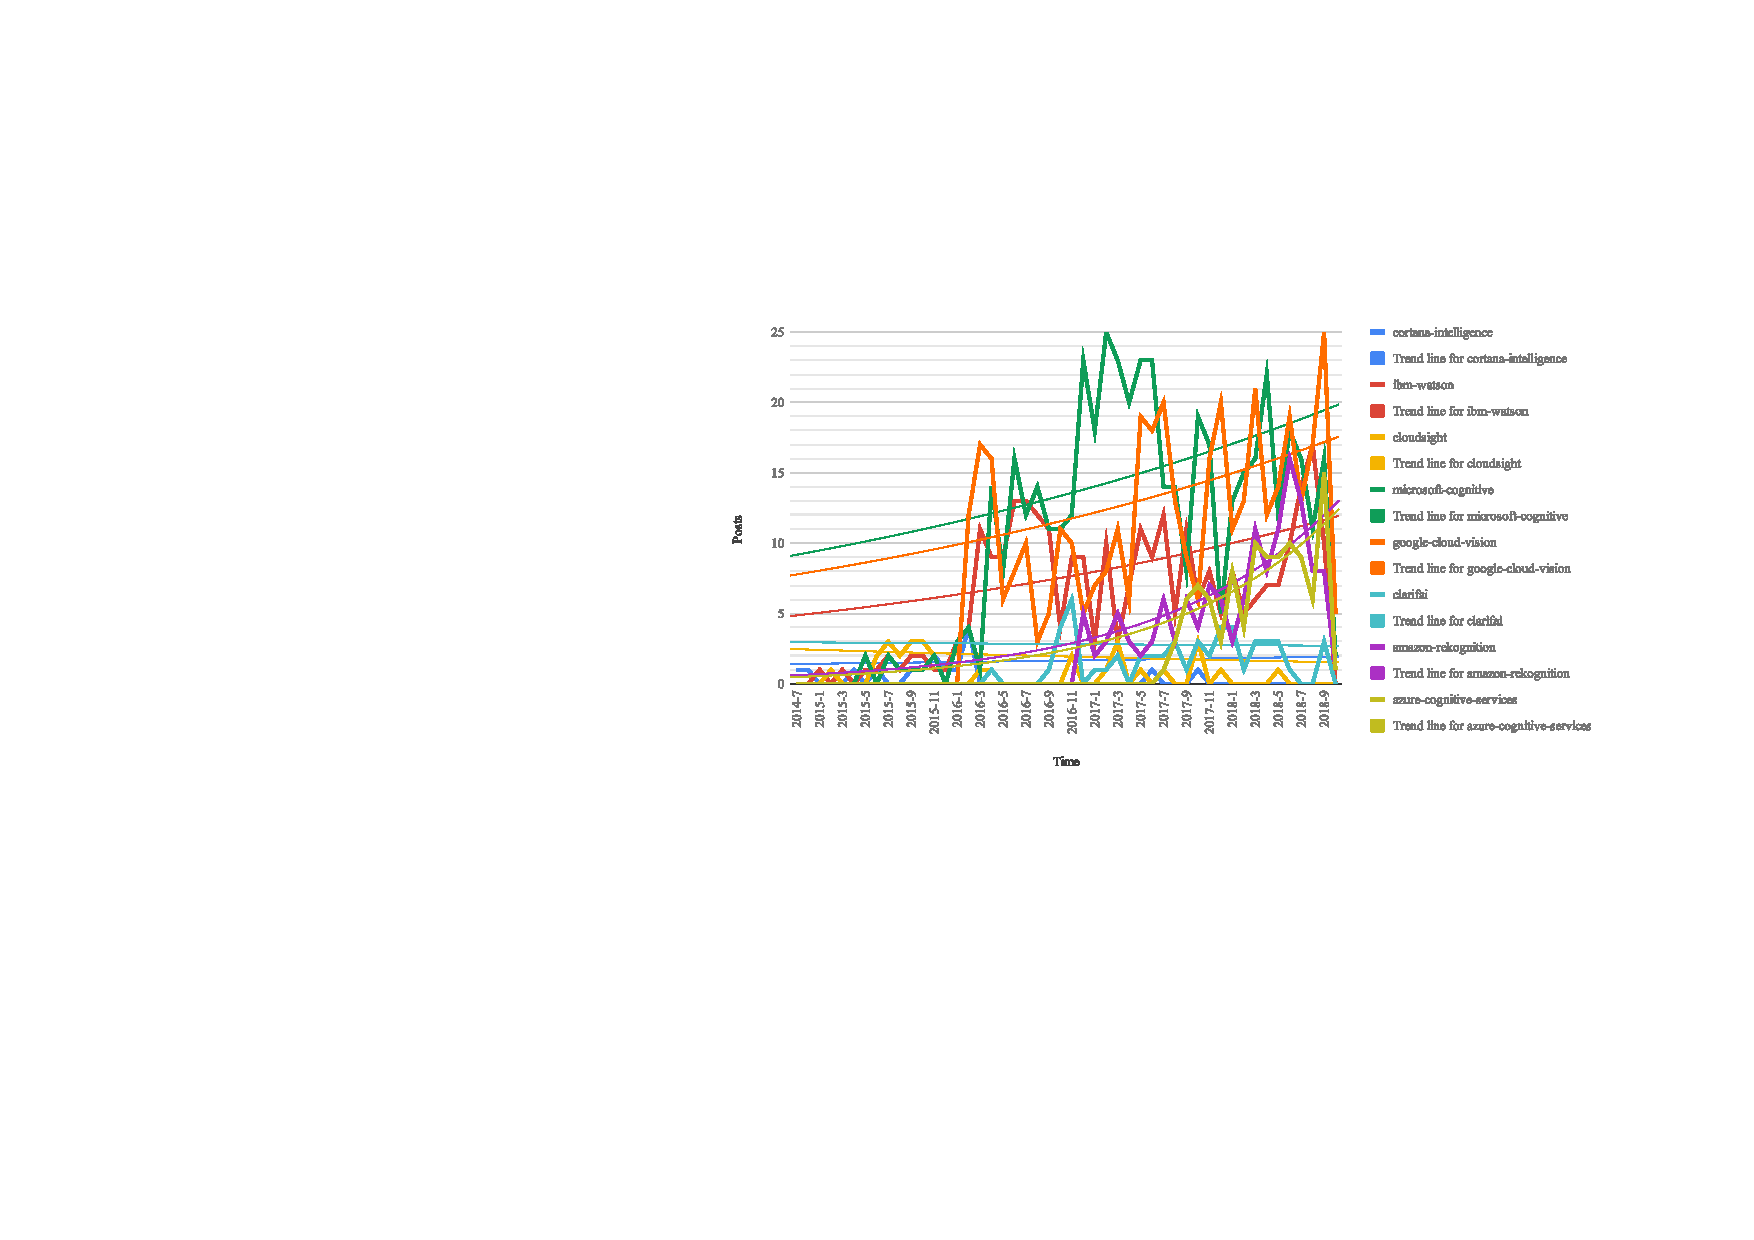
\includegraphics{stackoverflow-trends}
\end{figure}

\begin{figure}[th]
\centering
\caption[Overview of cloud intelligence services]{Overview of Cloud Intelligence Services.}
\label{fig:introduction:cloud-intelliegnce-service}
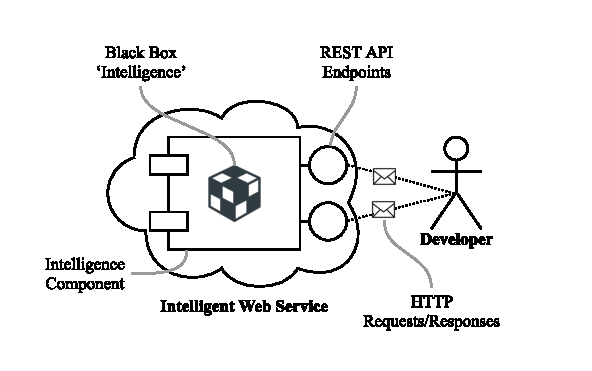
\includegraphics{cloud-intelliegnce-service}
\end{figure}

 
The general workflow of a \gls{cis} is relatively simple: a developer accesses a \gls{cis} component via REST/SOAP API(s). For their given input, they receive an intelligent-like response typically serialised as JSON/XML. We note the intelligence component masks its `intelligence' through a black-box: in recent years, there is a rise in providing human-level intelligence via crowdsourcing Internet marketplaces such as Amazon Mechanical Turk~\citep{MTurk:Home} or ScaleAPI~\citep{ScaleAPI:Home}. Thus, a \gls{cis} may be powered by varying degrees of intelligence: human intelligence, machine learning, data mining or even intelligence by brute-force.

While there are many types of \glspl{CIS} evident (such as OCR transcription, text-to-speech and speech-to-text, object categorisation, object comparison, natural language processing etc.), we scope the work investigated in this study to computer vision \gls{cis} analysers~\citep{GoogleCloud:Home,Azure:Home,AWS:Home,Pixlab:Home,IBM:Home,Cloudsight:Home,Clarifai:Home,DeepAI:Home,Imagaa:Home,Talkwaler:Home,Kairos:Home,Cognitec:Home,Affectiva:Home}. The ubiquity of computer vision \glspl{cis} is exemplified through evermore growing applications that use these APIs: aiding the vision-impaired \citep{Reis:2018cp,daMotaSilveira:2017vp}, accounting  \citep{Marshall:2018uj}, data analytics \citep{Iyengar:2017fb}, and student education \citep{Dibia:2017iy}. Moreover, we refer to its growing adoption in developer circles within \cref{fig:introduction:stackoverflow-trends}.